\documentclass{standalone}
\usepackage{tikz}
\usetikzlibrary{shapes, arrows.meta}

\begin{document}

% Economics Bar Chart: GDP Growth by Sector

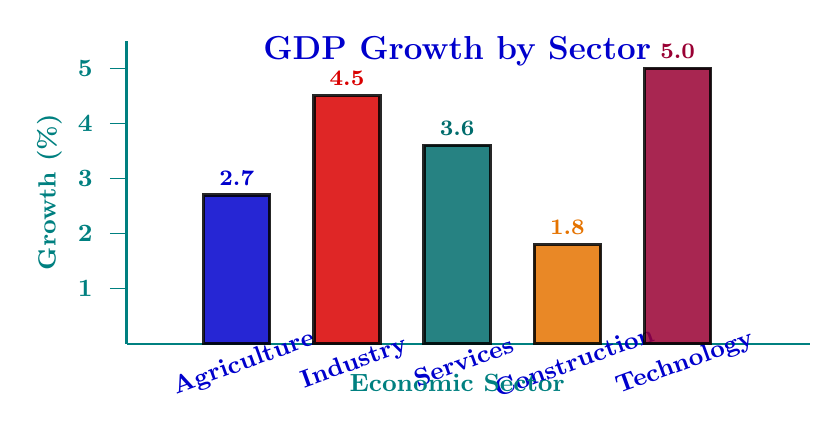
\begin{tikzpicture}[x=1.4cm, y=0.7cm]
  % Axis
  \draw[thick, teal] (0,0) -- (6.2,0);
  \draw[thick, teal] (0,0) -- (0,5.5);

  % Y-axis labels
  \foreach \y in {1,2,3,4,5}
    \draw[teal] (-0.15,\y) -- (0,\y);
  \foreach \y in {1,2,3,4,5}
    \node[left, font=\small\bfseries, teal] at (-0.22,\y) {\y};

  % X-axis labels
  \foreach \x/\name in {1/{Agriculture},2/{Industry},3/{Services},4/{Construction},5/{Technology}}
    \node[below, font=\small\bfseries, blue!80!black, rotate=20] at (\x,0) {\name};

  % Bars
  \draw[fill=blue!80!black, opacity=0.85, draw=black, line width=1.2pt] (0.7,0) rectangle (1.3,2.7); % Agriculture
  \draw[fill=red!85!black, opacity=0.85, draw=black, line width=1.2pt] (1.7,0) rectangle (2.3,4.5); % Industry
  \draw[fill=teal!85!black, opacity=0.85, draw=black, line width=1.2pt] (2.7,0) rectangle (3.3,3.6); % Services
  \draw[fill=orange!90!black, opacity=0.85, draw=black, line width=1.2pt] (3.7,0) rectangle (4.3,1.8); % Construction
  \draw[fill=purple!80!black, opacity=0.85, draw=black, line width=1.2pt] (4.7,0) rectangle (5.3,5.0); % Technology

  % Values atop bars
  \node[font=\footnotesize\bfseries, above, blue!80!black] at (1,2.7) {2.7};
  \node[font=\footnotesize\bfseries, above, red!85!black] at (2,4.5) {4.5};
  \node[font=\footnotesize\bfseries, above, teal!85!black] at (3,3.6) {3.6};
  \node[font=\footnotesize\bfseries, above, orange!90!black] at (4,1.8) {1.8};
  \node[font=\footnotesize\bfseries, above, purple!80!black] at (5,5.0) {5.0};

  % Title
  \node[font=\bfseries\large, blue!80!black] at (3,5.3) {GDP Growth by Sector};

  % Axis labels
  \node[font=\bfseries\small, teal, rotate=90] at (-0.7,2.75) {Growth (\%)};
  \node[font=\bfseries\small, teal] at (3,-0.7) {Economic Sector};
\end{tikzpicture}

\end{document}